% Upload this .tex file together with the sibling images/ directory to Overleaf.
% The figures below are already generated and referenced where they should appear.

\documentclass[11pt]{article}

\usepackage[margin=1in]{geometry}
\usepackage[T1]{fontenc}
\usepackage[utf8]{inputenc}
\usepackage{graphicx}
\usepackage{booktabs}
\usepackage{float}
\usepackage{hyperref}
\usepackage{xcolor}
\usepackage{tabularx}
\usepackage{array}
\usepackage{enumitem}
\usepackage{setspace}
\usepackage{caption}

\graphicspath{{images/}}
\setstretch{1.08}
\setlength{\parskip}{0.45em}
\setlength{\parindent}{0pt}

\hypersetup{
  colorlinks=true,
  linkcolor=blue,
  urlcolor=blue,
  citecolor=blue
}

\title{\textbf{CS 4365/6365 Final Project Report}\\[0.4em]
Agentic AI Sports Analytics Assistant}
\author{Sanjay Maddala \and Ryan Capozzi}
\date{Spring 2026}

\begin{document}

\begin{titlepage}
    \centering
    {\Large Georgia Institute of Technology\par}
    \vspace{0.5em}
    {\large CS 4365/6365: Intro to Enterprise Computing\par}
    \vspace{2.5em}
    {\Huge \textbf{Final Project Report}\par}
    \vspace{0.6em}
    {\LARGE Agentic AI Sports Analytics Assistant\par}
    \vspace{2.5em}
    {\large Team Members: Sanjay Maddala, Ryan Capozzi\par}
    \vspace{0.5em}
    {\large Term: Spring 2026\par}
    \vfill
    {\large April 26, 2026\par}
\end{titlepage}

\tableofcontents
\clearpage

\section{Introduction}
Sports analytics tools often fall into one of two weak patterns: either they are static dashboards with fixed filters, or they expect the user to already know SQL, Python, or spreadsheet-style analysis. Our project addresses that gap by building an agentic NBA analytics assistant that accepts natural-language questions, resolves the intended entities and metrics, generates safe database queries, executes them against historical game and player data, and returns grounded analyst-style conclusions.

The system is intentionally designed around verifiable analytics rather than free-form text generation. Every answer is meant to be backed by query results, with explicit provenance, constrained SQL, and a response layer that emphasizes conclusions, evidence, and caveats. That design choice became the main differentiator of the project: the goal was never only to ``translate English into SQL,'' but to make the resulting answer feel like a compact basketball analysis note.

\section{Motivation}
The motivation for this project comes from two practical problems. First, many basketball questions are analytical rather than lookup-oriented. Users do not simply want a table; they want a conclusion such as whether a team's win rate improves under a scoring threshold, whether one franchise has recently outperformed another, or whether a player's season-by-season profile reveals a meaningful trend. Second, the path from raw historical CSV data to such an answer usually requires too many steps for a casual user.

This project therefore focuses on a middle ground between traditional sports dashboards and unconstrained large-language-model agents. We wanted a system that remains deterministic where possible, but still feels conversational and useful. In that sense, the most important deliverable is not only the NL-to-SQL path, but the reasoning layer on top of it: ambiguity handling, safe execution, grounded summarization, and clear analytical conclusions.

\section{Related Work}
This project sits at the intersection of sports analytics, text-to-SQL systems, and safe data-grounded AI assistants. Prior work in text-to-SQL has demonstrated that natural-language interfaces can significantly lower the barrier to structured data access, especially when the schema and intent are well specified \cite{spider}. At the same time, deploying these ideas in practice requires schema-aware validation and strong query guardrails, which is one of the reasons we adopted SQL rewriting and validation rather than unrestricted generation.

On the implementation side, our system also draws from practical toolchains rather than only benchmark literature. The repository uses PostgreSQL as the execution engine, SQLGlot for parsing and validation, and Matplotlib for charting representative outputs \cite{sqlglot,postgresql,matplotlib}. The project therefore emphasizes end-to-end systems integration: data ingestion, query planning, execution safety, analytical narration, and reproducible local evaluation.

\section{System Architecture}
\subsection{Pipeline Overview}
The architecture follows a template-first approach. A user question is passed through intent classification and entity resolution, then converted into a structured query specification. The primary path uses deterministic SQL builders for supported query families, while an LLM-based fallback remains available for cases that do not match a known pattern. Before execution, every query passes through a guardrail layer that blocks unsafe statements, restricts table access, and adds row limits.

After execution, the result set is summarized by an insight generator that prefers deterministic, factual summaries and only uses a rewrite/review layer when the generated wording preserves the underlying numbers. This is the layer that turns raw output into short analyst-style answers. The CLI then prints the answer together with SQL, provenance, and top rows.

% Overleaf asset: images/system_architecture.png
\begin{figure}[H]
    \centering
    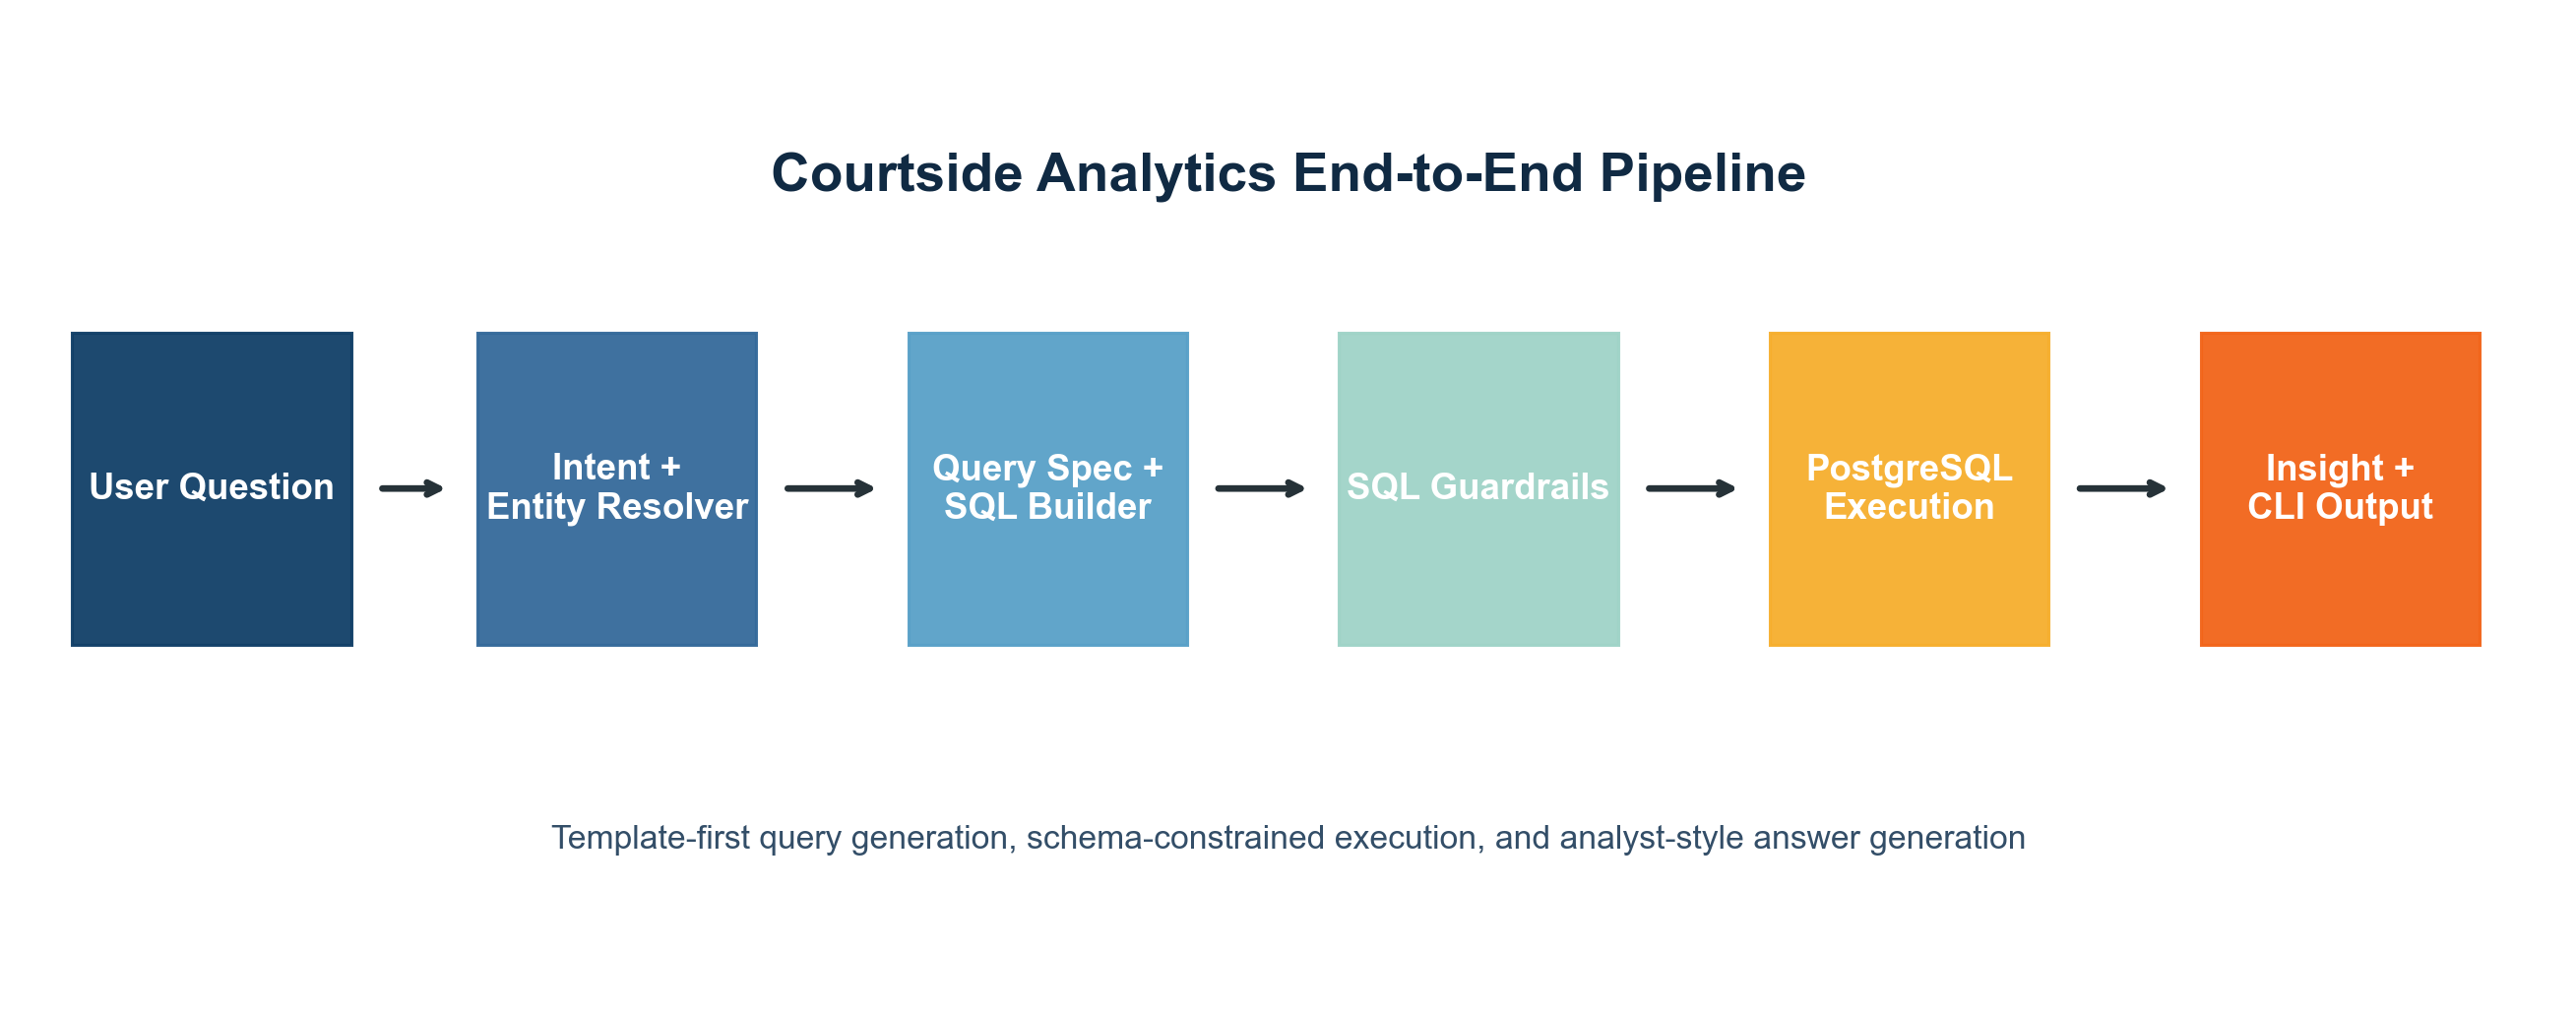
\includegraphics[width=\textwidth]{system_architecture.png}
    \caption{End-to-end architecture of the Courtside Analytics pipeline. The assistant is designed as a constrained analytics workflow, not a free-form chat system.}
    \label{fig:architecture}
\end{figure}

\subsection{Architecture Overview}
Where the pipeline overview explains the logical sequence of steps, the architecture overview explains the technologies that make those steps work in practice. The runtime path begins with a Typer/Rich CLI, flows through Python orchestration and agent modules, uses SQLGlot for SQL parsing and safety checks, executes against PostgreSQL, and optionally uses local Ollama models only at tightly controlled points such as fallback SQL generation or safe wording review. Matplotlib and the evaluation utilities sit beside the main query path so that the same grounded data flow can also produce charts, benchmark artifacts, and report-ready evidence.

Equally important is the way non-runtime materials support the architecture. The benchmark prompt set, regression tests, source-setup notes, and demo runbook do not answer user questions directly, but they are part of the overall system because they make the project verifiable, explainable, and reproducible for someone who did not build it.

% Overleaf asset: images/technology_architecture_overview.png
\begin{figure}[H]
    \centering
    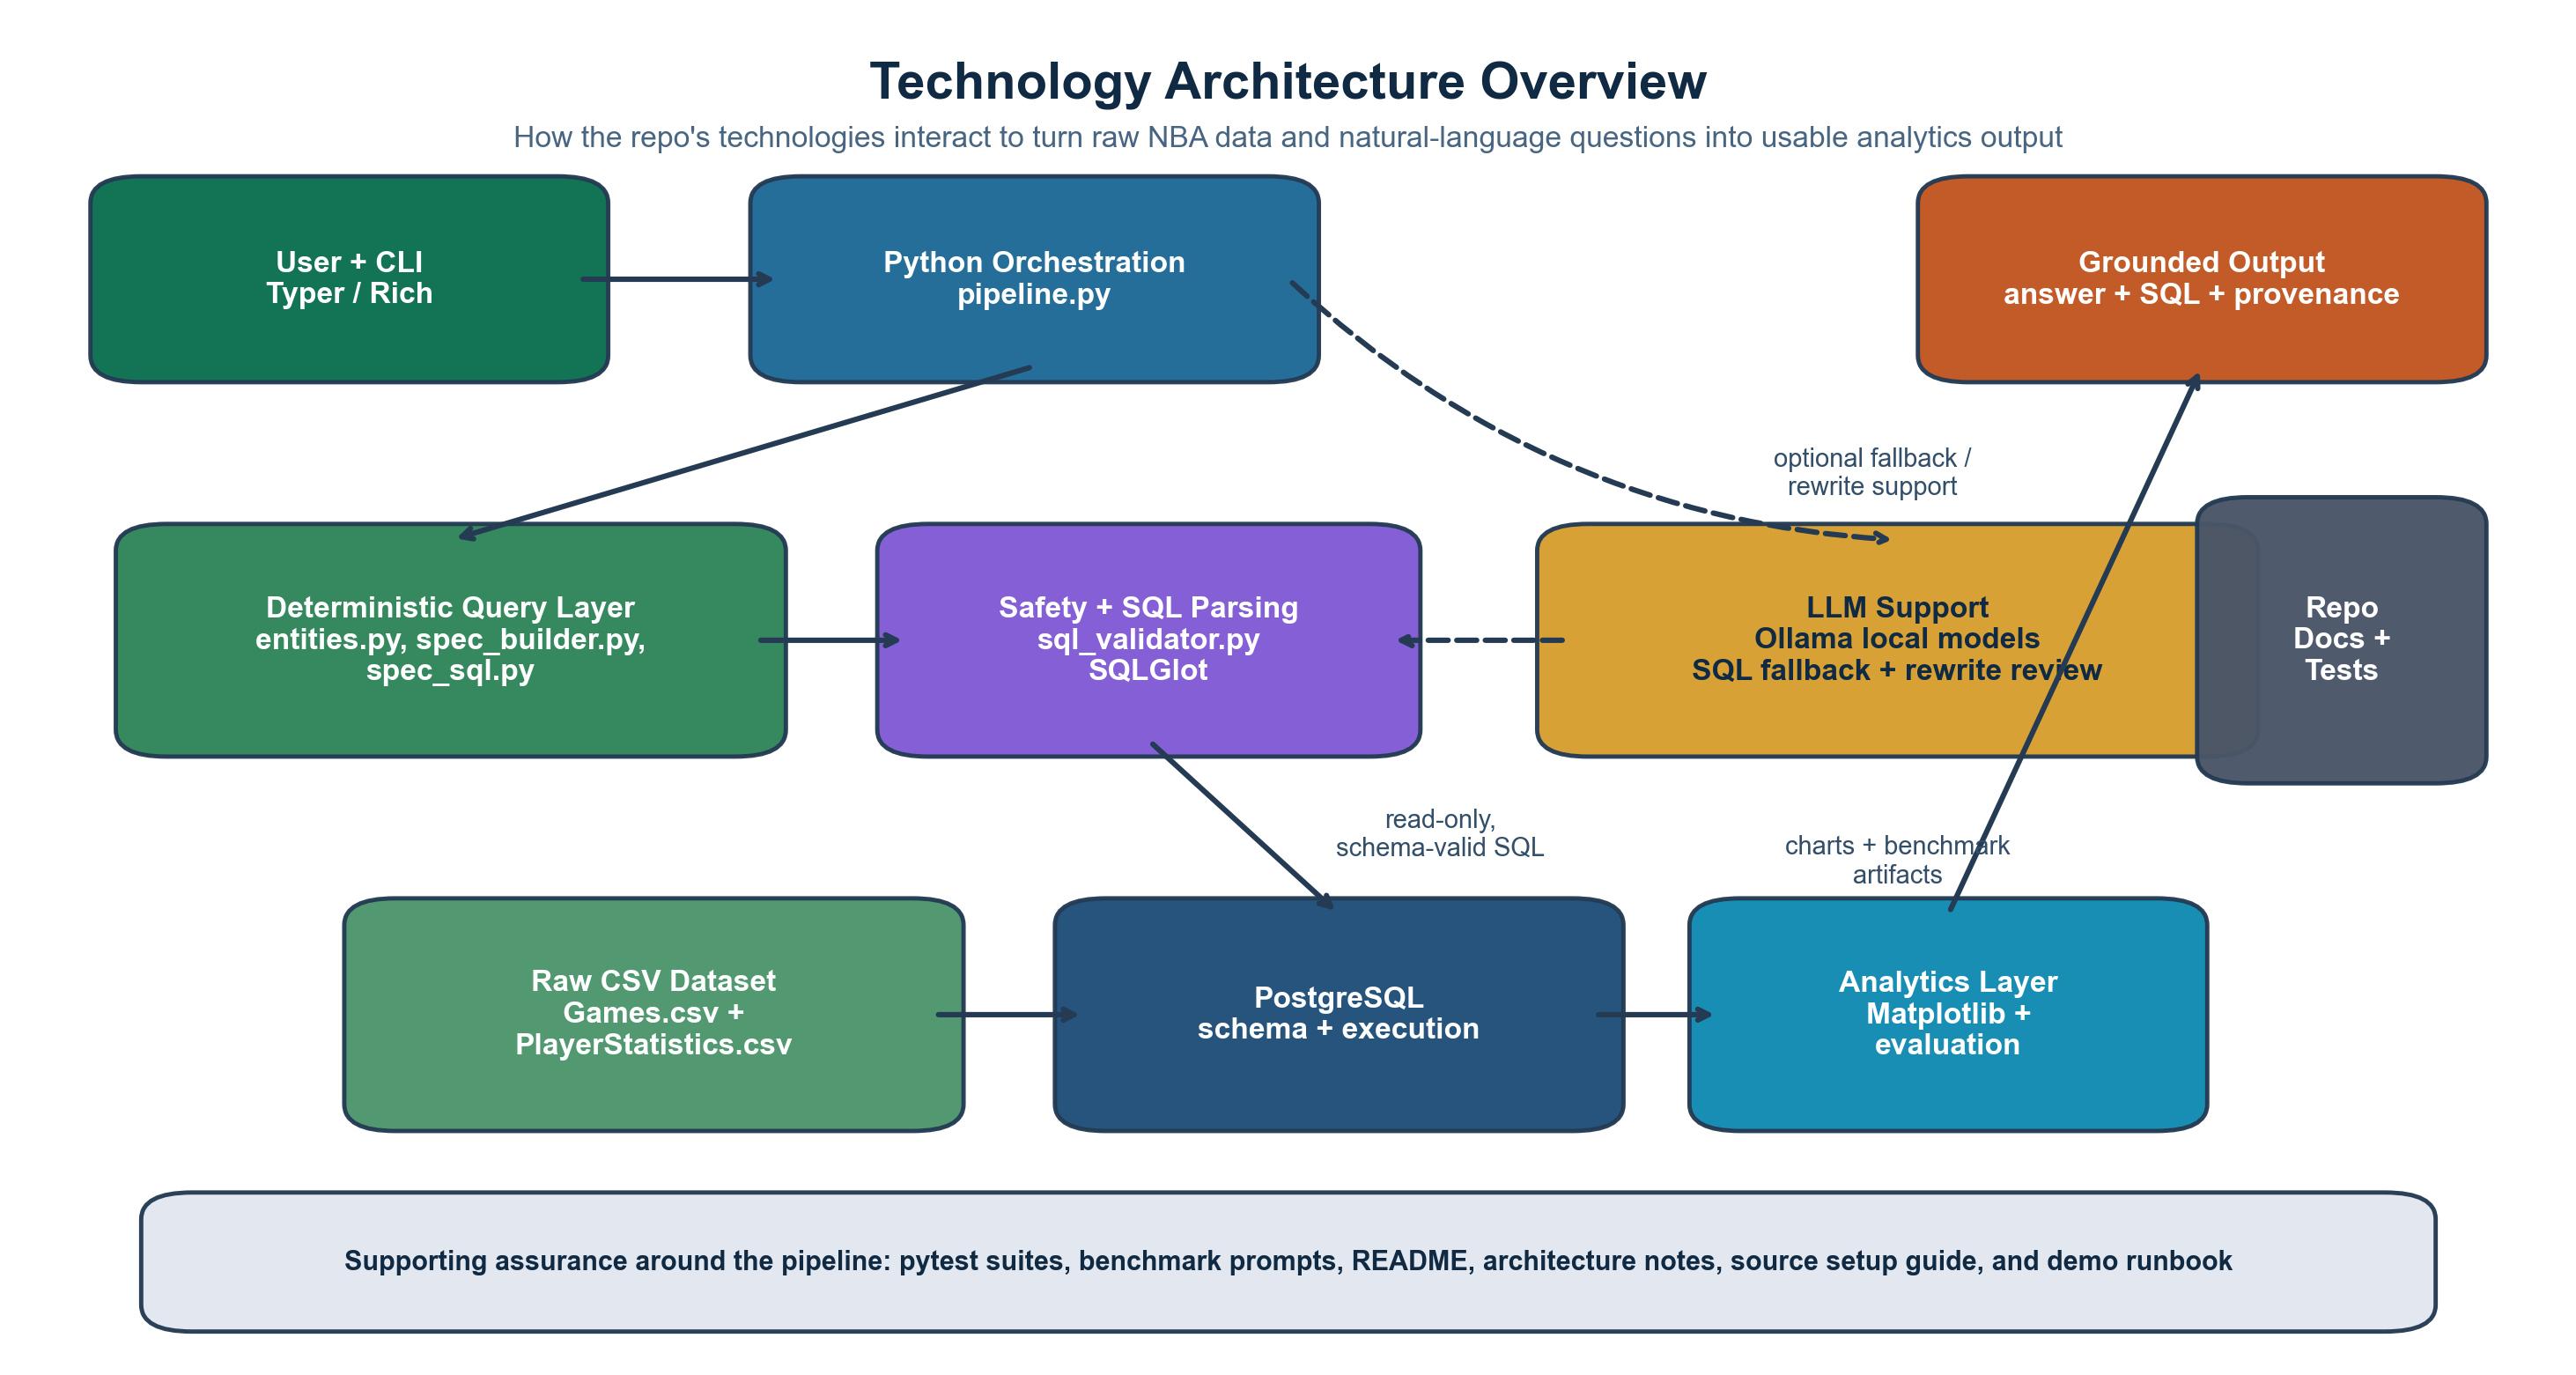
\includegraphics[width=\textwidth]{technology_architecture_overview.png}
    \caption{Technology architecture overview showing how the repository's tools, services, and validation materials interact with the pipeline to produce grounded and usable analytics output.}
    \label{fig:technology-architecture}
\end{figure}

\subsection{Safety and Reasoning Layers}
Two design choices are especially important for the final deliverable. First, ambiguity is treated as a first-class concern. If a question is missing a critical player or team reference, the agent now stops and asks for clarification before it attempts query planning. Second, the answer layer is built to foreground interpretation. The report-ready version of the system explicitly emphasizes conclusion, supporting evidence, and caveats instead of returning bare SQL results or generic summaries.

This matters because a sports analytics assistant should not merely produce data; it should help a user understand what the data implies. In practice, that means describing win-rate changes, identifying leaders, comparing seasons, and noting when a sample is narrow or partially complete.

\section{Dataset and Statistics}
The project uses a local historical NBA CSV workflow centered on \path{games.csv} and \path{player_game_stats.csv}. These inputs are validated and profiled before ingestion. On the local dataset used for this report, the repository recognizes 72,994 games and 1,662,378 player-game-stat rows covering 80 seasons, from November 26, 1946 through March 18, 2026.

\begin{table}[H]
    \centering
    \caption{Dataset and validation summary used for this report.}
    \label{tab:dataset-summary}
    \begin{tabular}{@{}ll@{}}
        \toprule
        Metric & Value \\
        \midrule
        Historical games & 72,994 \\
        Player-game-stat rows & 1,662,378 \\
        Coverage window & November 26, 1946 to March 18, 2026 \\
        Distinct seasons & 80 \\
        Benchmark questions & 30 \\
        Regression suites & 13 \\
        Latest full pytest run & 118 passed cases \\
        \bottomrule
    \end{tabular}
\end{table}

The figure below summarizes two important aspects of the dataset: recent season coverage and the distribution of game types. The visible dip in 2011--12 corresponds to the lockout-shortened season, while the incomplete 2025--26 count is expected because the local data snapshot ends on March 18, 2026 rather than after the full season.

% Overleaf asset: images/dataset_overview.png
\begin{figure}[H]
    \centering
    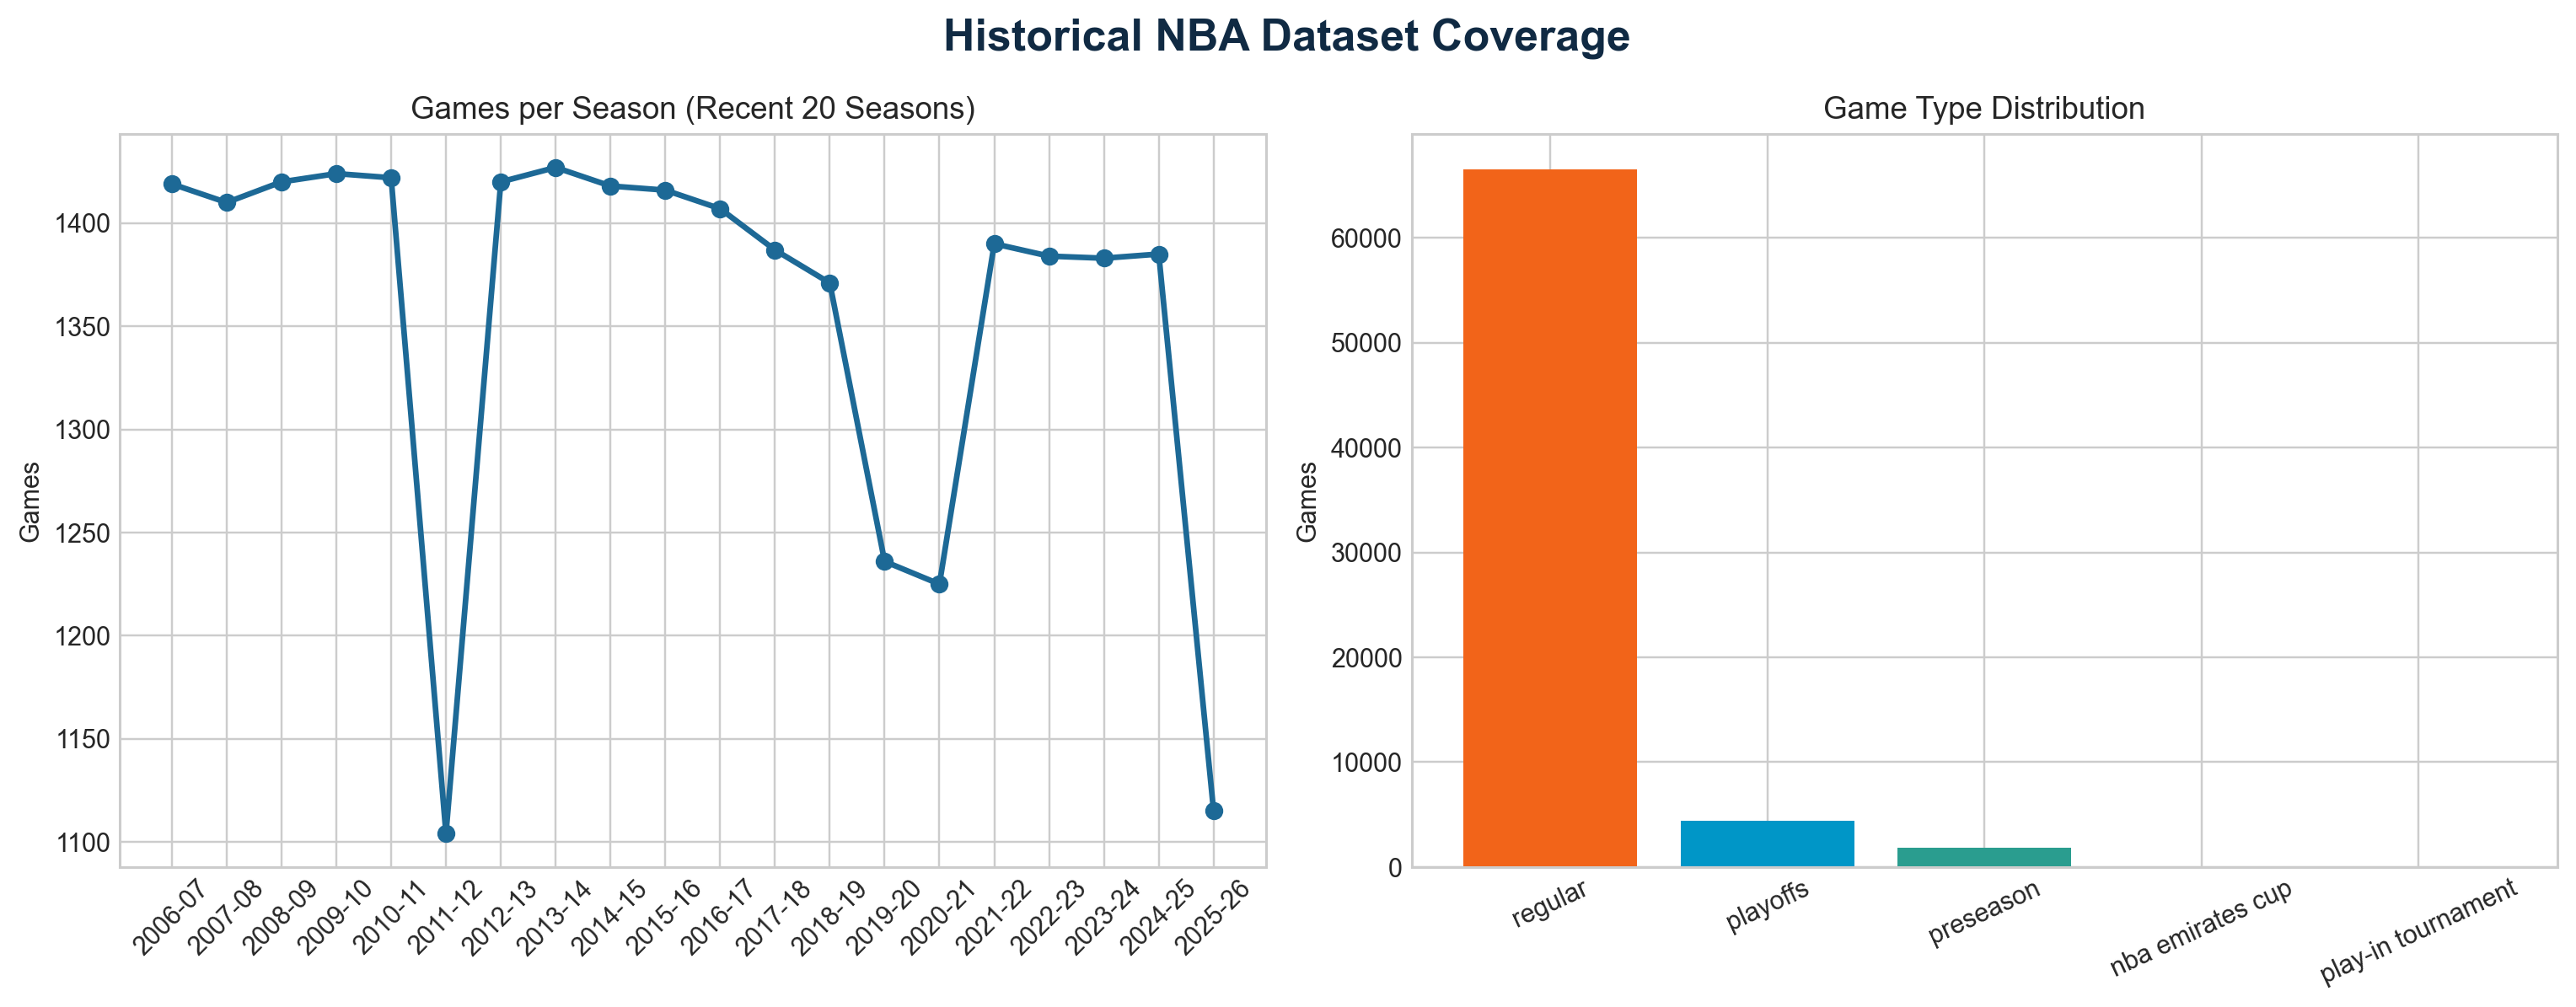
\includegraphics[width=\textwidth]{dataset_overview.png}
    \caption{Historical dataset coverage derived from the local raw CSVs. The left panel shows recent season game counts; the right panel summarizes the dominant game-type categories captured by the project data pipeline.}
    \label{fig:dataset-overview}
\end{figure}

\section{Implementation Methodology}
\subsection{Data Ingestion and Normalization}
The ingestion layer accepts multiple source naming conventions and maps them into canonical column names using alias tables and normalization utilities. This makes the project more portable across collaborators and avoids brittle assumptions about raw CSV schemas. The ETL path also derives missing season labels from dates, derives teams and players when optional reference files are absent, and performs sanity-preserving row drops for records that cannot be joined safely.

\subsection{Query Understanding and SQL Generation}
The agent pipeline is centered on explicit query specifications. Instead of hard-coding intent classification directly into template branching, the system first resolves entities, thresholds, season scope, metric choice, grouping, and response mode into a structured \texttt{QuerySpec}. That intermediate representation makes the system easier to debug, easier to test, and more faithful to the actual intent of the user question.

\subsection{Execution Safety and Insight Generation}
The SQL layer uses deterministic builders for supported families such as conditional team performance, player rankings, team comparisons, and season trends. Queries are validated with SQLGlot-based guardrails before execution. The insight layer then transforms query results into analyst-style summaries. This stage is especially important for the final deliverable because it is where the project moves from ``database interface'' to ``analytics assistant.''

\subsection{Repository Footprint}
The repository footprint reflects that systems focus. The largest code surface lies in the agent and testing layers, followed by ingestion, database utilities, and analytics support. This balance is deliberate: for a project that must be factual and safe, correctness and regression coverage are as important as feature count.

% Overleaf asset: images/artifact_footprint.png
\begin{figure}[H]
    \centering
    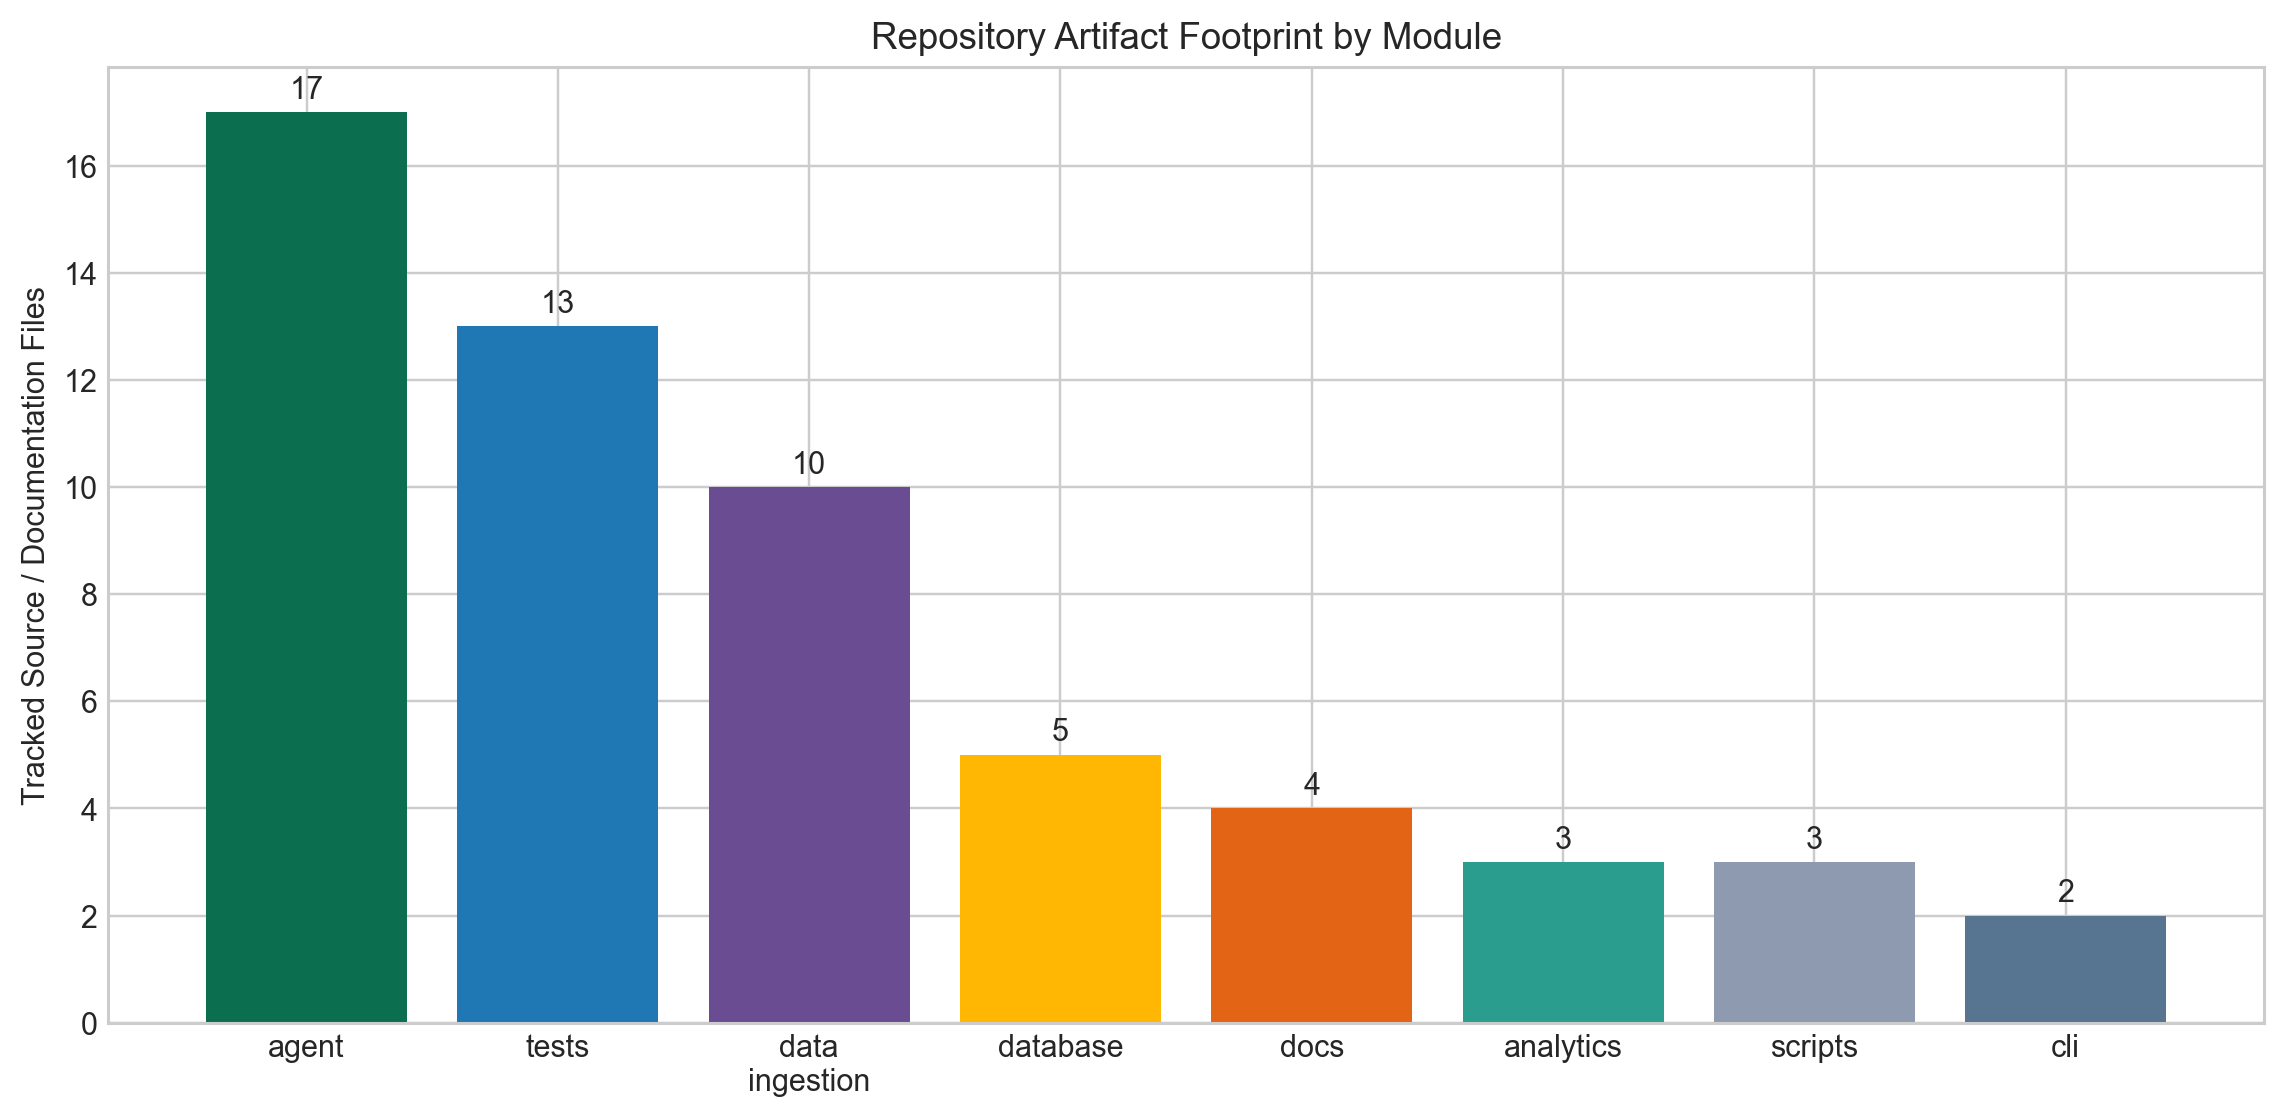
\includegraphics[width=0.88\textwidth]{artifact_footprint.png}
    \caption{Tracked implementation footprint by module. The agent, tests, and data-ingestion layers account for most of the repository effort.}
    \label{fig:artifact-footprint}
\end{figure}

\section{Evaluation and Results}
\subsection{Validation Strategy}
The evaluation strategy combines a benchmark harness with regression testing. The benchmark set contains 30 natural-language prompts spanning the four supported question families currently emphasized by the system: conditional team performance, team comparison, team trend, and player ranking. In parallel, the regression suite validates intent extraction, entity resolution, query-spec generation, SQL safety, insight wording, visualization behavior, CLI paths, and evaluation/report formatting.

As of April 26, 2026, the repository passed 118 pytest cases. In addition, the benchmark harness is integrated into the CLI and produces structured JSON and Markdown artifacts when the local database and model services are active. This means the final deliverable includes not only the agent itself, but also the reproducible evaluation path needed to demonstrate and inspect it.

% Overleaf asset: images/validation_overview.png
\begin{figure}[H]
    \centering
    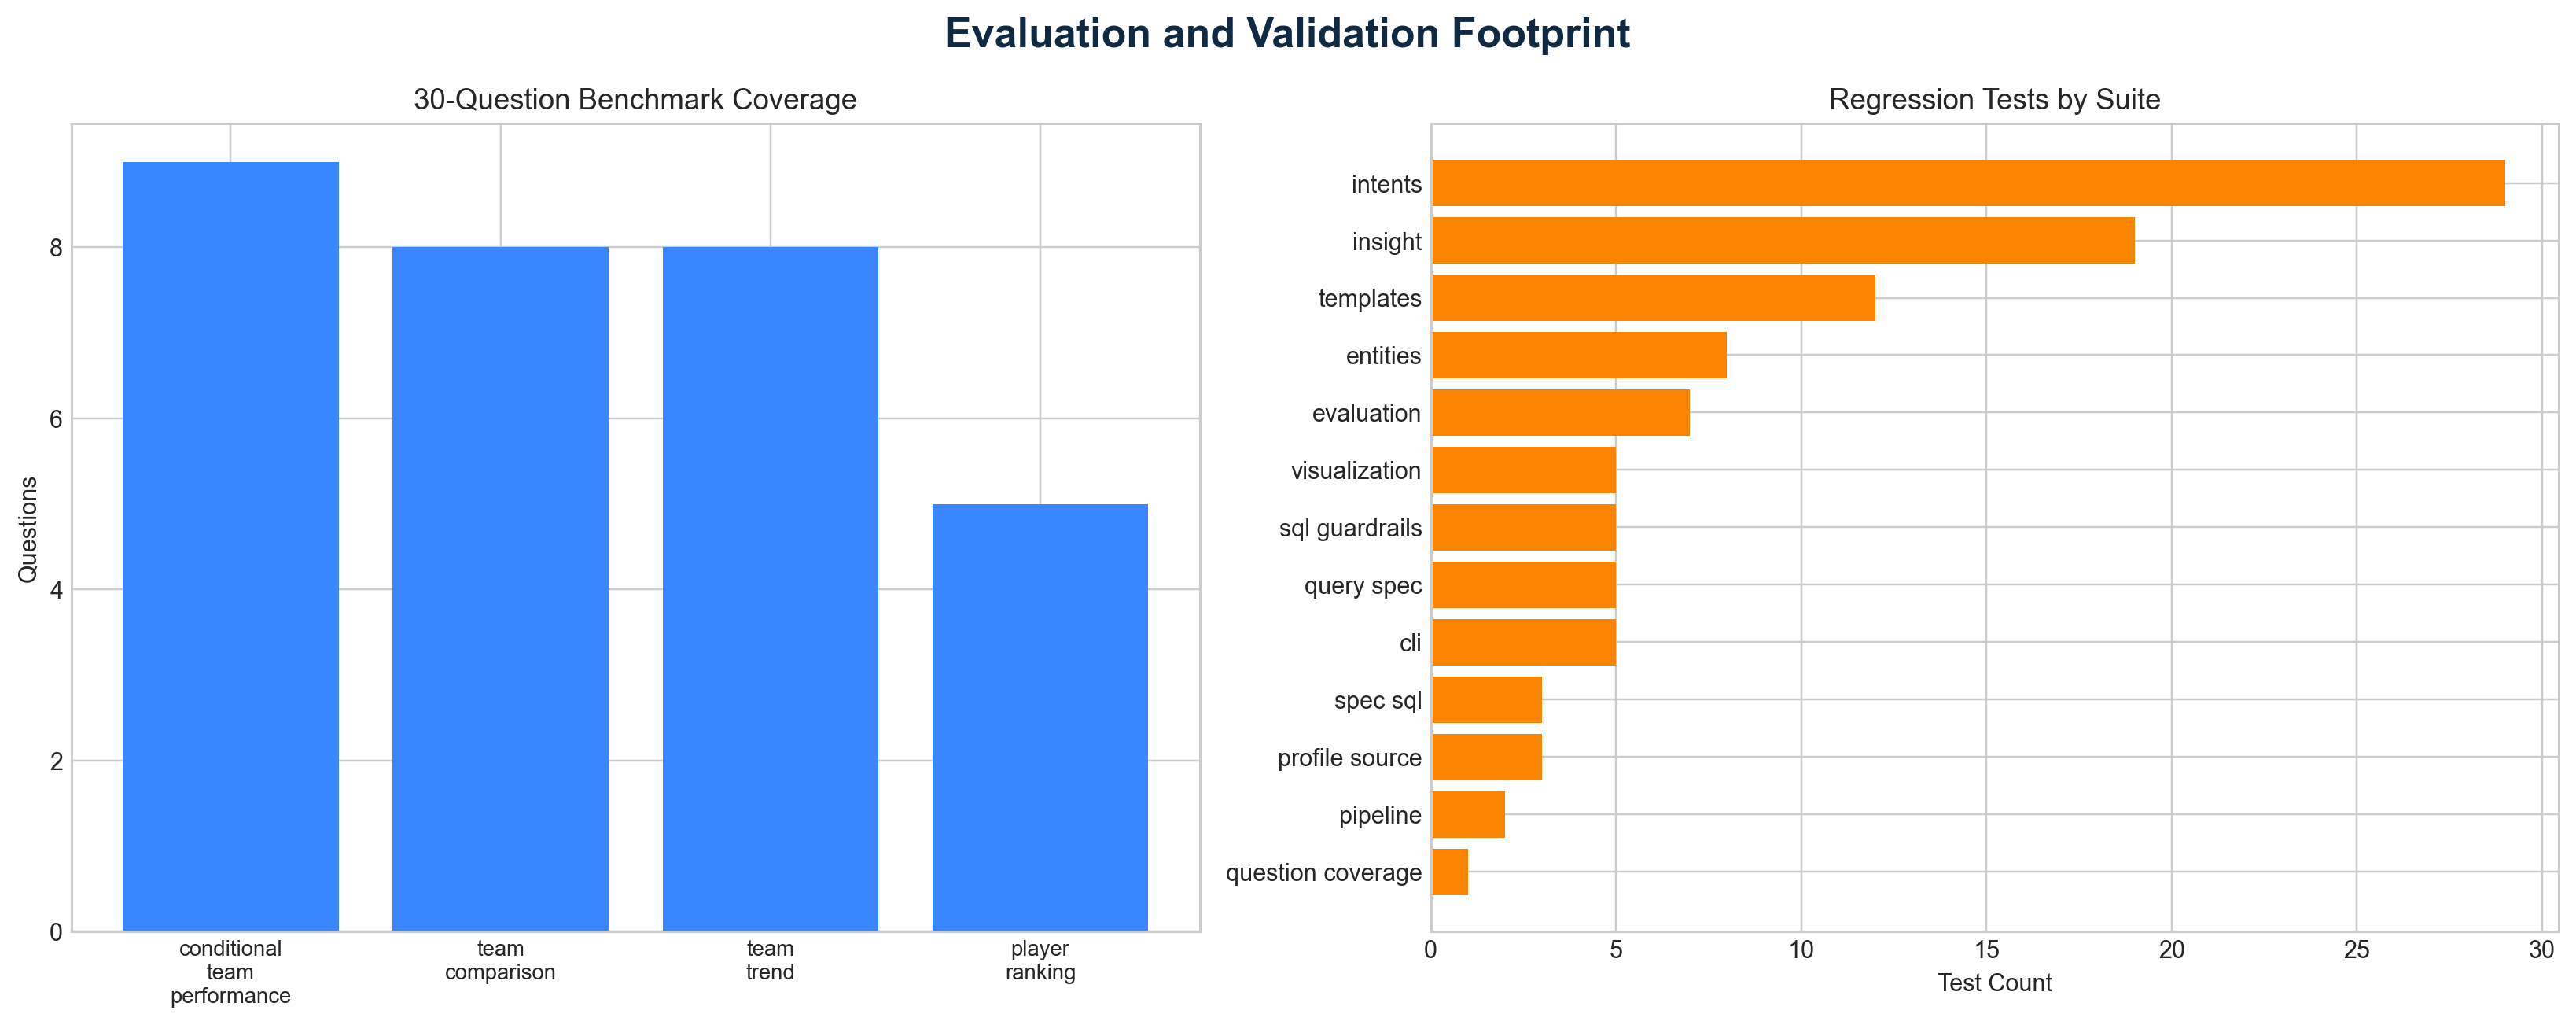
\includegraphics[width=\textwidth]{validation_overview.png}
    \caption{Evaluation coverage from the repository itself. The benchmark prompt mix provides breadth across core query families, while the regression suite provides depth across implementation layers.}
    \label{fig:validation-overview}
\end{figure}

\subsection{Representative Analytical Output}
To demonstrate the type of output the system is designed to support, Figure~\ref{fig:team-demo} visualizes a representative comparison query using the historical game data directly. Over the recent window shown, the Lakers peaked at 73.24\% regular-season win percentage in 2019--20 and reached 63.77\% in the partial 2025--26 snapshot, while the Warriors peaked at 81.71\% in 2016--17 and sit at 47.83\% in the current partial season snapshot. This is exactly the kind of evidence the assistant is expected to turn into a concise comparative conclusion.

% Overleaf asset: images/team_trend_demo.png
\begin{figure}[H]
    \centering
    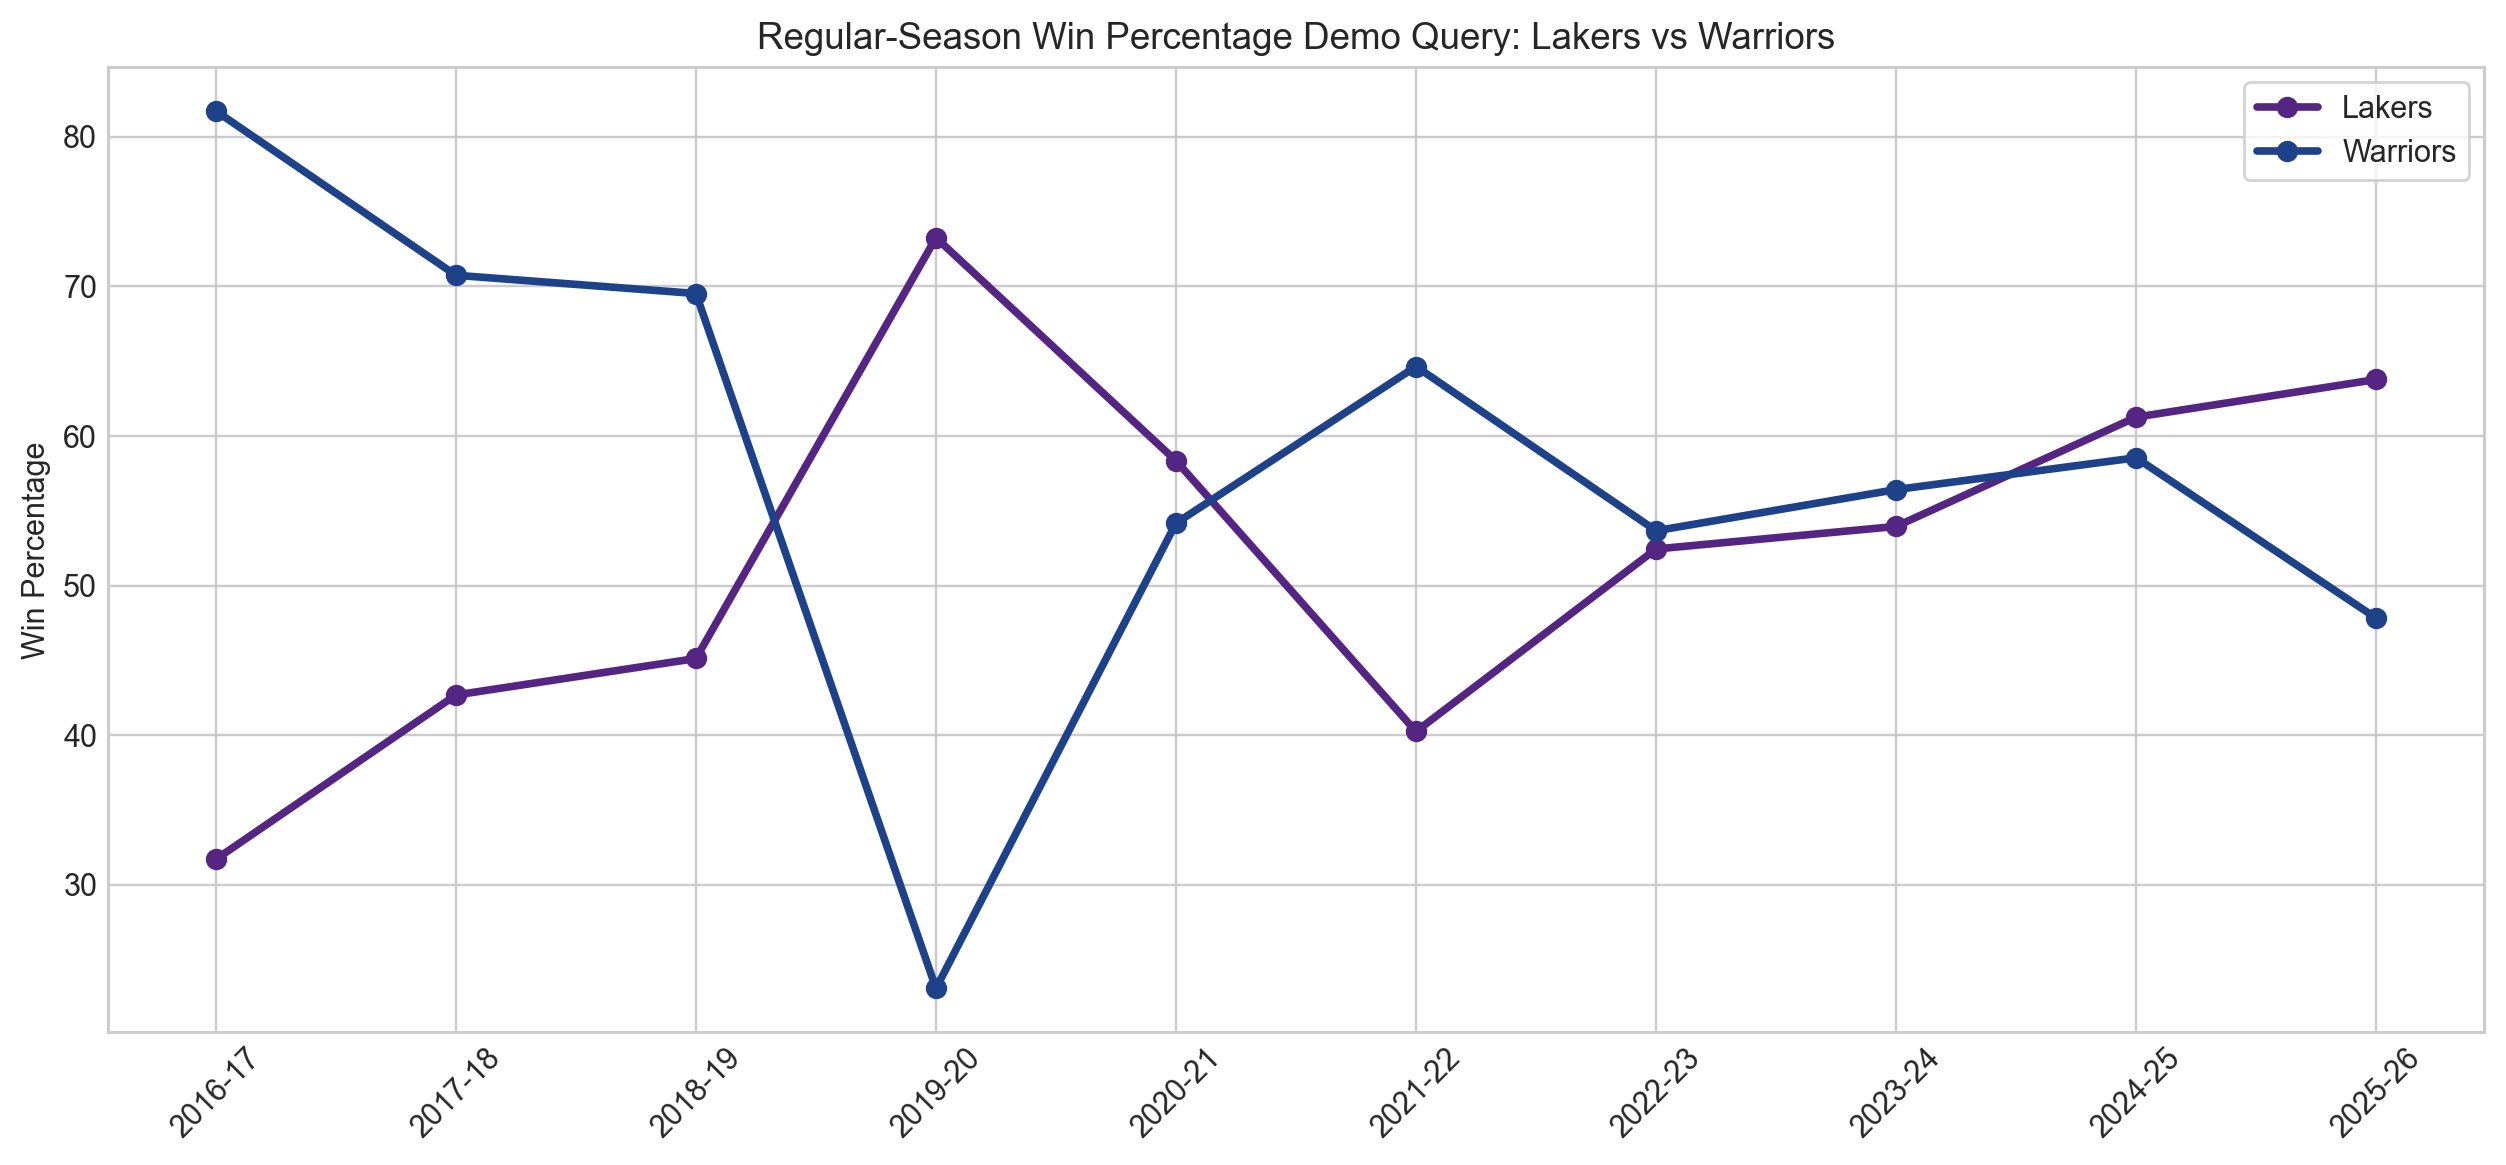
\includegraphics[width=\textwidth]{team_trend_demo.png}
    \caption{Representative analytics output derived from the project dataset: regular-season win-percentage comparison for the Lakers and Warriors across recent seasons.}
    \label{fig:team-demo}
\end{figure}

\section{Challenges Faced}
\subsection{Data Heterogeneity and Long-Horizon Coverage}
One of the earliest challenges was that historical NBA data is not cleanly packaged for direct analytics use. Source files use different naming conventions, optional reference tables are not always available, and some fields that are important for analysis, such as season labels or canonical entity names, must be derived or normalized. Because the project spans data from 1946 through 2026, even small inconsistencies can multiply across many decades of records. A substantial portion of the work therefore went into designing ingestion logic that was resilient to source variation without silently corrupting the final database.

\subsection{Balancing Flexibility with Safety}
A second challenge was finding the right boundary between flexibility and control. Natural-language questions vary widely in phrasing, but allowing unconstrained SQL generation would have made the system much harder to trust and debug. The project therefore had to support a conversational user experience while still prioritizing deterministic query building, schema-aware validation, and explicit clarification behavior when a prompt was underspecified. Getting that balance right was one of the hardest architectural decisions in the project.

\subsection{Producing Conclusions Instead of Bare Results}
Another challenge was moving beyond the easy demo of ``question in, SQL out.'' A useful sports analytics assistant should not stop at a result table; it should tell the user what that result implies. That meant the answer layer had to do more than format rows. It had to express a conclusion, preserve exact numbers, mention the analytical basis for the conclusion, and acknowledge caveats such as partial seasons or limited sample size. Building that reasoning layer in a way that stayed grounded to actual query results was a meaningful challenge and a major focus of the final deliverable.

\subsection{Reproducibility Across Local Services}
The final challenge was operational rather than algorithmic. The project depends on local data files, a PostgreSQL instance, a Python environment, and a local Ollama runtime. That creates multiple points where a demo can fail even if the underlying code is correct. To address that, the repository needed not only implementation code but also setup instructions, audit commands, evaluation commands, and a demo runbook. In other words, submission readiness required us to think about the project as a package that another person could run, not just as code that worked on one machine.

\section{Conclusion}
The final system is a functioning, repository-backed NBA analytics assistant with a clear architecture, repeatable ingestion path, SQL safety layer, analyst-style answer generation, scoped visualization support, and strong regression coverage. The project succeeded in moving beyond a proof-of-concept NL-to-SQL pipeline and into a more reliable analytics workflow that is easier to explain, test, and demonstrate.

Most importantly, the final deliverable now better reflects the real goal of the project: not just letting a user ask a question in natural language, but helping the user receive a grounded basketball conclusion backed by actual data and accompanied by enough context to understand what the result means.

\section{Future Work}
There are several meaningful next steps. First, the benchmark harness could evolve from a reproducible workflow into a routine release artifact so that each demo snapshot is accompanied by fresh summary outputs. Second, the system could support a broader set of query families such as head-to-head team histories, player threshold counts, and richer player profile narratives. Third, the visualization layer could expand from scoped season-based charts into a broader set of analytical plots once the supported shapes are better standardized.

Longer term, the assistant would also benefit from a lightweight web interface, more explicit user-facing clarification loops, and stronger evaluation tied to answer quality rather than only query success. These extensions would strengthen the product experience without weakening the core commitment to factual, constrained analytics.

\section{Deliverables}
The final repository contains the following deliverables:
\begingroup
\sloppy
\begin{itemize}[leftmargin=1.5em]
    \item \textbf{PostgreSQL schema and audit tooling:} \path{database/schema.sql}, \path{database/setup_db.py}, \path{database/audit_db.py}, and \path{database/sanity_checks.sql}.
    \item \textbf{Repeatable ETL and data validation pipeline:} \path{data_ingestion/run_etl.py}, \path{data_ingestion/loaders.py}, \path{data_ingestion/profile_source.py}, and \path{docs/source_setup.md}.
    \item \textbf{Agent pipeline for natural-language analytics:} core modules including \path{agent/pipeline.py}, \path{agent/spec_builder.py}, \path{agent/spec_sql.py}, plus supporting entity and fallback logic.
    \item \textbf{Execution safety and answer grounding:} \path{agent/sql_validator.py} and \path{agent/insight.py}.
    \item \textbf{CLI demonstration workflow:} \path{cli/main.py} with \texttt{ask}, \texttt{evaluate}, \texttt{chart}, \texttt{check-data}, and database setup commands.
    \item \textbf{Evaluation and visualization support:} \path{analytics/evaluation.py} and \path{analytics/visualization.py}, backed by the curated 30-question benchmark in \path{data/benchmarks/questions.json}.
    \item \textbf{Regression coverage and project documentation:} the \path{tests/} directory together with the core writeups in \path{README.md} and \path{docs/}.
\end{itemize}
\endgroup

\section{Supporting Materials}
This report is the narrative entry point for the final deliverable, and the repository includes supporting materials that function as appendices for design, setup, evaluation, and demo use. These materials are important because they allow a reader to move from understanding the project conceptually to reproducing it in practice.

\begingroup
\sloppy
\begin{itemize}[leftmargin=1.5em]
    \item \textbf{Repository overview and quick-start guide:} \path{README.md} summarizes scope, setup, CLI usage, evaluation commands, and common troubleshooting steps.
    \item \textbf{AI-oriented execution guide:} \path{INSTRUCTIONS.md} is written so an AI agent can quickly understand the repository, set up dependencies and services, and run the full pipeline from data preparation through testing and CLI validation.
    \item \textbf{Architecture and design notes:} \path{docs/architecture.md} explains the system structure, technology choices, component interactions, and output contract.
    \item \textbf{Source-data setup guide:} \path{docs/source_setup.md} documents the accepted raw CSV filenames, loading expectations, and audit workflow.
    \item \textbf{Live demo instructions:} \path{docs/demo_runbook.md} provides a step-by-step sequence for starting services, loading data, asking representative questions, running the benchmark workflow, and showing a chart during the demo.
    \item \textbf{Planning and quality targets:} \path{docs/plan_v4.md} records the locked scope, milestone sequence, and quality bar that guided the final implementation.
    \item \textbf{Evaluation inputs and report assets:} \path{data/benchmarks/questions.json}, \path{report/images/}, and \path{scripts/generate_report_assets.py} provide the benchmark prompt set, the figures used in this report, and the script used to regenerate those figures.
\end{itemize}
\endgroup

\section{Skill Learning}
This section focuses on the course-relevant skills we developed through the project rather than a list of isolated technologies. The strongest takeaway from this work is that enterprise-style computing depends on disciplined scoping, interface design, evidence, and communication just as much as it depends on implementation ability.

\subsection{Scoping and Constraint Management}
One of the most important skills we learned was how to define and protect scope. Early in the project, it would have been easy to chase a much broader vision for sports analytics, but the final deliverable improved once we locked the problem around game-level NBA analytics, a template-first query path, local-model support, and a benchmarkable set of question families. Learning to commit to those constraints, and to treat them as design tools rather than limitations, was a major project-management skill developed through the semester.

\subsection{Systems Thinking Across Boundaries}
The project reinforced that real systems work is about the interactions between layers, not just the quality of any one layer in isolation. A natural-language analytics assistant only feels coherent when the data contract, schema, query planner, SQL validator, execution engine, insight generator, and CLI all agree on what the system is supposed to do. We became much better at tracing failures across boundaries and recognizing that an issue that looks like a ``model problem'' may actually be a schema, ETL, or interface-definition problem.

\subsection{Designing for Trust Rather Than Novelty}
Another important skill learned was how to prioritize trustworthiness over novelty. A more unconstrained agent might appear more impressive at first glance, but for this project we learned to value behaviors that make outputs safer and more defensible: clarification when the prompt is ambiguous, deterministic SQL where possible, explicit guardrails, and answers that are tied back to evidence. That shift in mindset, from ``what can the system generate?'' to ``what can the system responsibly support?'', is one of the most valuable course-related lessons from the project.

\subsection{Evidence-Driven Iteration}
We also strengthened our ability to measure progress through artifacts rather than intuition. Tests, benchmark prompts, audit commands, report figures, and demo instructions all became part of how we judged whether a feature was actually complete. This made us more careful about distinguishing between something that was partially implemented, something that was reproducible, and something that was ready to present. That habit of evidence-driven iteration is directly transferable to future enterprise and AI systems work.

\subsection{Interface Design, Ownership, and Collaboration}
The project improved our ability to create clean working boundaries between collaborators. Moving toward explicit structures such as a query specification layer, separate validation modules, and clearly documented setup steps made it easier to divide work without losing coherence. We learned that good collaboration is not only about communication frequency; it is also about designing interfaces, responsibilities, and handoff points that reduce ambiguity for other contributors.

\subsection{Technical Communication as Part of the Deliverable}
Finally, the project strengthened our ability to present technical work as a complete deliverable rather than a pile of source files. Writing checkpoints, improving documentation, assembling supporting materials, and shaping this final report all required us to explain decisions, tradeoffs, and evidence in a structured way. That skill is especially important in enterprise settings because the value of a system is often judged first through its documentation, reproducibility, and clarity before anyone studies the implementation details.

\section{Task Breakdown}
\begin{table}[H]
    \centering
    \caption{High-level task breakdown for the final deliverable.}
    \label{tab:task-breakdown}
    \begin{tabularx}{\textwidth}{@{}>{\bfseries}p{0.2\textwidth}X@{}}
        \toprule
        Team Member & Primary Contribution Areas \\
        \midrule
        Sanjay Maddala & Final report assembly, evaluation framing, data-validation workflow verification, deliverable packaging, and systems-level integration checks across the project. \\
        Ryan Capozzi & Query-spec refactor, deterministic SQL generation, visualization path, CLI workflow support, and recent correctness improvements across the analytics pipeline. \\
        Shared Work & Repository documentation, regression testing, schema and ETL design, ambiguity handling, insight-generation refinement, and end-to-end architecture decisions. \\
        \bottomrule
    \end{tabularx}
\end{table}

\begin{thebibliography}{9}

\bibitem{spider}
Tao Yu, Rui Zhang, Kai Yang, et al.
\newblock Spider: A Large-Scale Human-Labeled Dataset for Complex and Cross-Domain Semantic Parsing and Text-to-SQL Task.
\newblock In \emph{Proceedings of EMNLP}, 2018.

\bibitem{sqlglot}
Toby Mao, et al.
\newblock SQLGlot: Python SQL Parser, Transpiler, and Optimizer.
\newblock \url{https://github.com/tobymao/sqlglot}

\bibitem{postgresql}
The PostgreSQL Global Development Group.
\newblock PostgreSQL Documentation.
\newblock \url{https://www.postgresql.org/docs/}

\bibitem{matplotlib}
John D. Hunter.
\newblock Matplotlib: A 2D Graphics Environment.
\newblock \emph{Computing in Science \& Engineering}, 9(3):90--95, 2007.

\end{thebibliography}

\end{document}
